\chapter{Methodology \label{ch3}}

The following chapter will detail the methodological decisions taken for the development of this research, as well as a quick outline of the theoretical framework that
supports the ideas and procedures followed, the analysis strategy and the constraints and limits identified in the methodology proposed.

The first section will focus on the research strategy, the philosophical background used to support the decisions taken, the approach selected for the research design, and
the limits and constraints imposed by those decisions. The second section will explain the most important elements of the theoretical framework that supports this research,
considering that this project uses both, an educational research lens and a software development.

In the educational field, this research uses as foundation the views proposed by social constructionism of how knowledge is built and the effect of social interactions and
cultural context in the educative process. The collaborative learning approach uses those fundamentals to propose methodologies for learning design, assessment and analysis.

Finally, the technical approach will detail the process used for the design, development and evaluation of \emph{WorkshopAR}, emphasising the design philosophy followed to
involve as much as possible the input of the user. This approach is used to better integrate the learning design (of this project and of the target course) into the
development of the software. This can be evidenced in the design exercises proposed for the interaction with the functionalities, the overall user experience and the
discovery of functional requirements.

\section{Research Strategy \label{sec:3-1}}

This project is qualitative and exploratory in nature. Qualitative because at the core of the research questions, there is the idea of description. The goal is to describe
behaviours and characterise the technology selected as it is used in the classroom. It is exploratory because, rather than trying to corroborate or to formulate a theory,
the goal is to gather enough data to understand the characteristics of the scenario being studied. This will allow to formulate a way forward to deeper analysis of the
issues and questions that stood out through the review of relevant literature and previous experiences in the field.

\ac{CR} was identified as a good fit for the philosophical approach of the research. Observation will be at the core of the enquiry process and the data gathered will be
subjective in nature, linked to very specific points of view: the observations of the researcher, the perceptions of students and teaching staff. \ac{CR} proposes an
approach to research that takes into consideration the imperfections inherent to understanding reality through such subjective perceptions, finding value in identifying
and gathering different views of the same issue \parencite{hastings_2021,bryman_2003}.

Since very specific points of view are going to be the main source of analysis, it is important to understand and accept that any data and observation will be flawed and
that all results proposed, especially those that try to identify the underlaying mechanisms in the social phenomena observed, will be in need of interpretation and
contextualisation to assess validity or applicability beyond the case study here exposed \parencite{easton_2010}.

Section \ref{sec:2-2-4} explores the tendency found in literature on justifying any educational development through improvements in average grades or similar gains, to
give the research validity using a very positivistic framework of analysis, while neglecting or obscuring the human and social core of education. CR offers a midpoint
between positivism and social constructionism by acknowledging the social dynamics used to build knowledge and learning processes, the ontological framework used to model
and interpret qualitative data as well as linking all these ideas with a more empirical understanding of the mechanism working underneath what is observed \parencite{parra_2021}.

Both \textcite{carter_2004, scott_2005} highlight that one of the most important tools in \ac{CR} research is to identify agency and structure, that is, to understand the
phenomenon being observed by identifying who is doing things, what are the social connections at play and the reasons behind the actions being observed. This approach
requires the presence of both empirical, hard data that can be analysed, as well as the necessity for a more interpretative and qualitative approach to those elements that
cannot be described with just numbers.

\ac{CR} is also a framework well suited to answer \emph{how} and \emph{what} questions. \textcite{wang_2021} explains that the Empirical-Actual-Real model used in \ac{CR}
(see Figure 1) can be used to explain ideas about causation, correlation and the underlying structures driving the empirical events we are experiencing. The research
questions proposed for this research both align to this view or were tuned to align with this approach. The main objective is to describe what is happening in the
classroom around the mechanisms of collaboration and the technological tools created as an engine of those mechanisms (the what, the empirical), and to create an
analytical and interpretative framework to explain those behaviours (the how, the actual). The research process will potentially identify a link between what was observed
with the ideas, designs and tools created.

\begin{figure}
    \centering{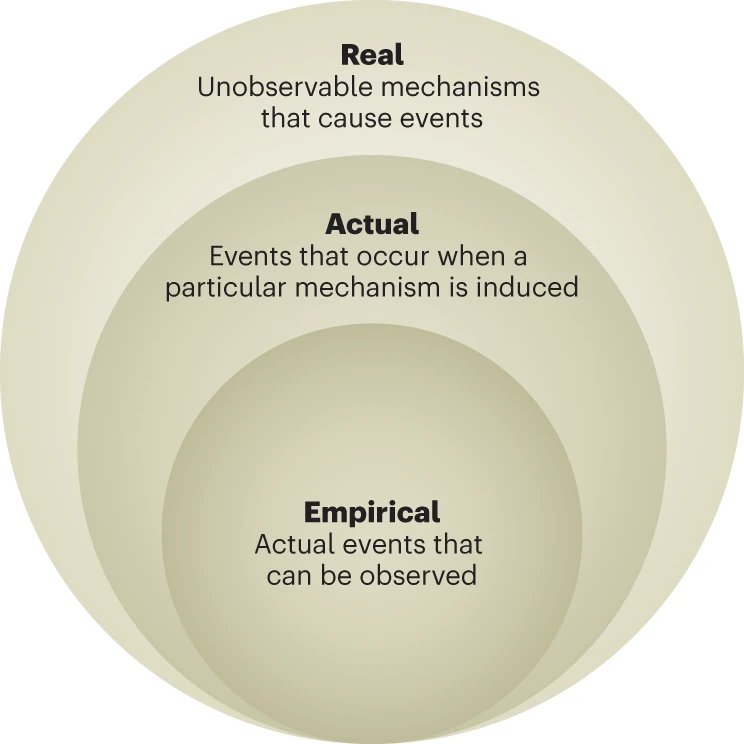
\includegraphics[scale=0.3,alt={Figure 3.1}]{figures/F3-1.jpg}}
    \caption{The Relationship Between the Real, the Actual and the Empirical \parencite{blackie_2023} \label{fig:3-1}}
\end{figure}

Given the emphasis on observational qualitative data, the best research type that fits the methodology so far described is an inductive approach. The main question (MQ) of
this research is aimed at understanding how \ac{AR} promotes observed behaviours, while questions SQ1 to SQ6 help describing the data with the goal of linking the
empirical data with the actual mechanisms in play throughout the educational scenario. The assumption here is that those mechanisms in fact exist, and that they are being
built or promoted using the technology that is part of the educational design of the activity.

It is important to clarify that the explorative nature of the data will not be totally blind. It will be informed by a series of expectations and hypothesis about how
\ac{AR} has been used in the past for educative scenarios and the theoretical background found in the literature about collaborative learning, project-based educational
design and \ac{TEL} experiences, all which were explored in Chapter \ref{ch2}. This background provides the biggest foundational ideas that will guide the analysis process
of the data:

\begin{itemize}
    \item \ac{AR} can be used in education as an effective tool for communication and it works by exploring the advantages inherent to the technology in the form of
    visualisation, interaction and connection with others.
    \item The core of collaborative learning lies in using social connections as the main driver of the educational design, and the main behavioural changes that could be
    observed will be present in those points where \ac{AR} is part of the social interactions taking place.
\end{itemize}

The analysis process will naturally try to find indications of those ideas in the data, mainly because it has been apparent in the results found in previous works. It is
also important to understand that the main research drive of this project is to identify all those elements that do not align with those ideas (if any), try to link them
to underlying mechanisms and refine those initial ideas based on what has been observed, and create a new or distinct starting point for future research.

Following the research strategy chosen, it was decided that a case study would fit best with the philosophy and research types adopted. This strategy offers a promising
approach to manage the kind of observations proposed, as the research is more interested in behaviours and personal perceptions and the way they change thanks to the
intervention designed. A detailed case study is well suited to create the scenario where these changes can be observed, even if it is difficult to identify and understand
all the variables and mechanisms operating behind the observed scenario.

Case studies produce the type of context-related knowledge that is most valuable in learning scenarios. They are also a very useful tool for contexts in which human
behaviour needs to be observed and in which a community is an integral part of the context \parencite{hamilton_2013}. Case studies are ideal tools to identify problems,
outliers and out of the norm observations. Moreover, thematics and problems characterised as rich or complex are perfect subjects for case studies, which have a good set
of tools to capture, organise and analyse extensive narratives, which value lies more on its density and richness rather than the factual data that can be extracted out of
it \parencite{seale_2007,grauer_2012}.

\textcite{cober_2015,tay_2017} represent example projects of educational case studies centred around a \ac{TEL} intervention. They demonstrate and set a precedent of many
of the foundations used in this research around technology in the classroom: a design process that involves the users and a feedback loop that adapts to the circumstances
observed. These examples also highlight some unique benefits of a case study approach like involving the community as an active part of the research, enriching the
discussion of the ideas generated by using different points of view and facilitating a two-way avenue of the benefits of the research, often allowing the researcher to
actively and directly make an impact on the community well beyond the research scope.

Finally, and given the prevalence of qualitative data in the research strategy selected, the analysis technique chosen for the project will focus on content and thematic
analysis. These approaches offer good flexibility to analyse the data obtained from different points of view that are subjective and anecdotal in nature. They help in
synthesising large quantities of textual data, organise them and extract relevant points of interest to start building results and conclusions \parencite{kiger_2020,neuendorf_2018}.
Specifically, the thematical analysis of the research will focus mostly on identifying themes related to:

\begin{itemize}
    \item The use of technology to manage team activities in the classroom.
    \item The prevalence and importance of technological tools while creating channels of communication among the groups.
    \item The interaction between the different tools used by the students.
    \item Instances of reflection and analysis of the activities in the classroom thanks to the use of the tool proposed for the intervention.
\end{itemize}

Although these themes are the focus of the analysis, it will be very important to track and identify any other relevant content that emerges during the observation phase,
especially if it is related to the collaboration process or the use of technology in the classroom. Additionally, these same analysis strategies can be used in the
evaluation process of the software development, offering a structured method to gather and analyse the qualitative data gathered about the usage of the tool and the
perceptions of the users while using it during the instances of controlled test and during the intervention in the classroom.

An important effort is also proposed to offer some triangulation to the data obtained from the case study. On one hand, the software development process requires a
substantial data analysis coming from the reported results of similar past projects and from the exercise in user-centred design that will be followed during the initial
stages of development of the tool. This process is also iterative in nature, and the feedback collected and analysed during the testing stages will inform not only the
development of the tool, but also the observation process.

A second approach for triangulation is the use of two extra data instruments to complement the observation process of the case study. One is focused on unstructured
interviews with the students with the objective of gathering data about their collaborative process, their approach to teamwork during the course and the tools they used
to make work possible or easier. The second instrument is a similar set of unstructured interviews focused on the teaching staff. These interviews will gather information
about the influence of teamwork and collaboration in the educational design of the course, the criteria used by the staff to assess a successful teamwork and their personal
views on how this project-oriented activities could be used to prepare the students for their professional lives.

\section{Research Constraints and Limits \label{sec:3-2}}

The biggest constraint on the timeline proposed for the development of this research is the access to the Industry Project course. Any cohort of the course runs through
two semesters, and it was important to follow the development of the project from the first contact the students have with the group to the final presentation of the
project. The observation window to achieve this objective is one academic year, which can be translated to 24 academic weeks along two semesters of 12 weeks in which
observation of the development of the course is possible.

This situation forces the project to adapt a cross-sectional approach, which tries to describe in as much detail as possible the effects observed of the technological
intervention for one cohort of the Industry Project course. The main objective is to create an internal comparison between those groups participating in the course as they
would normally do versus those using the \ac{AR} tool. As with most cross sectional studies, this approach offers a quick way of gathering data and the observations cover
multiple variables of interest that can be analysed later, at the cost of creating a situation in which the data will be biased to the particularities of this sample,
making it harder to propose any generalisation or causality \parencite{wang_2020}.

Sampling inside the cohort of the course will be guided by convenience and the disposition of the students to participate in the research, since it is important to
prioritise their academical work and minimise any disruptions to the classroom. Observations will be organised in singular work sessions that the students will be asked to
participate in. Each work session will be guided by the students, setting the goals of the session based on any requirements they have during that instance of development
of their project. The observation will try to focus on different aspects of the course that had not be observed previously. The researcher will also try to show the
students a different aspect of the \ac{AR} tool one functionality at a time, facilitating their involvement in the observation and helping with the iterative development
of the software. If possible, the observation will try to gather different work sessions focused on:

\begin{itemize}
    \item The initial contact and formation of the group.
    \item Understanding the project and gathering information about it.
    \item The initial design proposal and the flow of information between the different roles in the group.
    \item The creation of material for the project.
    \item Evaluation and correction of the material created based on the feedback of the teaching staff and their peers.
    \item A final evaluation of the work done by the group at the end of the project.
\end{itemize}

Ideally, the observations can gather instances of these activities for groups using the \ac{AR} tool and other groups working as they normally would. The observations
themselves will gather data of the student's work using mainly audio and video recordings, as well as the personal notes of the researcher. Data will be initially
organised based on the week it was taken (to determine the overall development stage of the course's project), the composition of the group observed and the functionality
of the \ac{AR} tool that was prioritised.

There are clear limits and constraints inherent to the research methodology chosen that are important to acknowledge and that will affect the results obtained:

\begin{itemize}
    \item Case studies are not well suited for generalisation and extrapolation \parencite{wiersma_2000,gerring_2004}. The results obtained through this project will be linked mainly to the case study selected
    and its unique characteristics. An important effort was done to select a case study that uses all the elements of collaborative learning needed for this research, as
    well as presenting a unique an interesting scenario which can provide insights usable in future research.
    \item The time constraints of the project cause the data points to reflect only one cohort of the course. Though it was possible to follow the whole development of the
    project, comparison among other cohorts would minimise the noise generated from difficulties and circumstances present in this instance of the course that could have
    affected in a negative way the observations obtained.
    \item The prototyping nature of the technological intervention also causes a lot of noise generated from the friction with learning and using the tool. This often is
    evidenced by observations that highlight the most comments and opinions of the tool around these disruptions and not the educational design.
    \item The predominance of qualitative data generated from this study needs to be interpreted and contextualised. In the same way, the focus on behaviour and underlying
    mechanism of social activities makes it impossible to create answers and observations that are not subjective in nature and marked by the biases of the researcher. An
    important effort is done to separate the observations from the analysis. The interpretation of the researcher will be well documented, but hopefully this research will
    also offer the opportunity for future work to recontextualise and propose different views to the data obtained and documented here.
\end{itemize}

Considering these constraints, it is important to follow the documentation of this project as an exercise in experimenting with the application of a unique technology in
the classroom, basing the evaluation method of the proposal on its observed effects in the learning process rather than in the assessment and end results. This is done in
hope of identifying good and bad influences that could be linked to the use of the technology proposed. In the end, the analysis of the results documented in this thesis
can be used as a starting point to develop similar experiences in the future in different contexts, either trying to emulate the same positive results or working on the
negative ones, inciting more discussions and pushing forward the understanding we have about the use of \ac{AR} technologies in the classroom.

\section{Theoretical Framework \label{sec:3-3}}

So far it has been explained that the approach to this research is through the themes and situations found in the classroom using two complementary fronts. This is first
and foremost an exercise in \ac{TEL}, with the firm idea in mind that it is impossible and neglectful to ignore the use of technology in the classroom. The first premise
that supports the proposal is that mobile technologies can be used in a positive and constructive way to promote learning and good behaviours, when used correctly and with
the proper guidance. The educational approach that guides the project focuses on the tools and theories that view education mainly as a social phenomenon and as an ongoing
construction based on our environment and experiences, as it will be explained in the following sections.

The technological development followed for this project also acknowledges the challenges found in the implementation of educational technology. The focus, besides a
successful implementation, is on executing and documenting the design process followed to create ideas and promote discussion about how to integrate the educational and
software design processes, how to align functional and learning goals and how to incorporate the students and the teaching staff into the process.

\subsection{Educational Approach \label{sec:3-3-1}}

The theoretical framework behind the educational proposal is in \ac{CL} used as a teaching tool to promote the communal construction of knowledge in the
classroom, to play with the strengths and flaws of both students and educators as well as facilitating the development of transversal skills such as teamwork and
communication.

\subsubsection{Collaborative Learning Structure \label{sec:3-3-1-1}}

\ac{CL} is seen as a philosophy of education that prioritises communal exploration over uniformity \parencite{eskiyurt_2024}. It assumes that learning is an
active process that depends on rich context, diversity and is inherently social \parencite{smith_1993}. In a collaborative design students benefit from a joint effort to
solve problems, a diversity of skills put together for a common purpose and a transmission, active and passive, of knowledge and skills between members of the group
\parencite{laal_2012,buchs_2015}.

\ac{CL} also goes beyond grouping students for an activity, it is an active educational design that seeks to integrate the learning goals of an activity into the dynamics
created in the group. \textcite{laal_2012} remarks the importance of creating positive interdependence between the members of a group, where the success of one individual
is linked to the success of all the others. This can only be achieved if the learning design allows for the group activity to create considerable and meaningful
interactions, mechanisms for personal responsibility, development of social skills, and spaces for the group to self-evaluate \parencite{johnson_1990}. \ac{CL} can be
distinguished from similar concepts like peer learning, tutoring and cooperative learning by the way it frames the relationship between students. It proposes an equal
relationship between peers that develops high levels of mutuality, that is, interactions that must be executed in both ways of the relationship \parencite{odonnell_2013}.

The education proposal of this research is founded on these characteristics. It is possible to summarise the goals of the TEL intervention with three objectives:

\begin{enumerate}
    \item Use the visual tools provided by \ac{AR} to reinforce ideas of interdependence and mutuality by highlighting important structures of the collaborative work such
    as roles, tasks and communal evaluation of progress.
    \item Leverage the communication features of a mobile deployment to provide extra channels for meaningful socialisation.
    \item Explore the concept of \emph{augmented collaboration} using visuals and interactions to give students a different way to approach elements of teamwork, team
    management and resource management.
\end{enumerate}

Paired with the requirements of the course, the learning activities that \emph{WorkshopAR} is meant to support are analytical and creative in nature, aimed at evaluating the
collaborative work of the students at a high cognitive level. If the design purpose of the tool is to provide a technological approach to develop the skills needed for an
effective collaboration, the observation stage of the project will evaluate if the students that are engaging with the tool are using it in a way that helped them with
these learning objectives, either:

\begin{itemize}
    \item To better organise or show the analysis done to the project through an understanding of the context of the problem, the use of their previous knowledge to
    propose a solution and communicating their analysis to their peers or the clients.
    \item As a tool that helps the creative activities needed for the proposed solution by pooling resources, help the discussion of ideas or approaches, help to organise
    tasks or keeping track of progress.
\end{itemize}

Observations of this type of activities, positive or negative, will be used to construct a satisfactory answer for the research questions, and will show that the tool is
indeed highlighting the aspects of collaborative work that are meant to be reinforced: organised and meaningful interactions plus a structured way to manage the
interdependent activities taking place in the group.

Available literature has also identified major obstacles that have to be acknowledged when proposing a \ac{CL} design. Section \ref{sec:2-1-4} highlighted the most
relevant literature found around this discussion. Other relevant work like the one present by \textcite{hansen_2006,pfaff_2003} also offer an important analysis of the
challenges found in collaborative settings that where critical in the design of \emph{WorkshopAR}. Of the ideas mentioned, it was considered important an interesting to emphasise:

\begin{itemize}
    \item The imbalances in dynamics, power and assessment that are often found in teamwork and how the students negotiate and work with them.
    \item The hurdles in communication that often are the focus of friction and failure in a team.
\end{itemize}

Finally, this is also an exercise in collaboration mediated by technology. There is ample discussion on the phenomena of online collaboration \parencite{hathorn_2002,rodchua_2017},
but the proposal of \emph{WorkshopAR} is to identify how this trend of asynchronous and discontinued communication is used outside the web and in the physical classroom, with the
main intention of identifying, if possible, positive or interesting behaviours that can be nourished to create a more positive relationship with technology inside the
classroom, akin to the proposals made by authors like \textcite{dyer_2015} or the analysis of available options and approaches from \textcite{olson_2012}.

\subsubsection{Social Constructionism \label{sec:3-3-1-2}}

If \ac{CL} is the central pillar of the educational proposal of this project, then social constructionism is at the core of the educational philosophy found in
collaborative learning. One of the main premises of social constructionism is that the cognitive development of people matures thanks to the guidance and collaboration
with others \parencite{rogoff_1990}. It is impossible to learn in complete isolation.

In this model of learning, communication is a key ingredient since language itself is the main driver for the construction of knowledge and the core medium for its
transmission \parencite{renzl_2007}. The immediate context, the cultural background, cultural artifacts, the relationships that had been build and the sense (or lack of)
pertinence to a group are all fundamental factors in the process of creating knowledge, and they are all inherently social \parencite{edley_2001,burr_2017}. It is no
surprise then that \ac{CL} echoes all these elements and bases most of its methodological approaches in social constructionism premises:

\begin{itemize}
    \item Focus on learning and working in small groups to facilitate the creation of meaningful relationships.
    \item A prevalence of discussions and debates as the main tool for the creation and transmission of knowledge.
    \item Use of tools that support communication.
    \item Guidance and mentoring as the primarily teaching intervention.
\end{itemize}

It is important to clarify that this research takes a stance in social constructionism and not in constructivism. The main reasoning follows the definitions used by
\textcite{rob_2018}. This research is focused more on the social aspects that can be observed in the case study, it is more interested in the behaviours of the group and
the way communal knowledge is built (which aligns better to the approach of constructionism) rather than the cognitive process of the individual interacting in the group
(a more constructivists view). In the end both terms are rather interchangeable and complementary, and both views agree in the fundamentals, but it is an important
distinction to establish and to keep consistent through the research.

Another important distinction is between weak and strong constructionism. The main difference lies in accepting the existence (or not) of \emph{brute facts}, absolute and
fundamental realities (weak constructionism), or rather considering that reality is completely created by social convention and interaction (strong constructionism)
\parencite{travers_2004,lawson_2002}. In its core, the distinctions are not fundamental for the proposal of this thesis, but a strong constructionist view aligns better
with the analytical methods proposed in the methodological design, since all observations are of social behaviours, and need to be filtered and understood through the
social context, cultural and linguistic frameworks of the case study. This also supports the view that any observation and analysis done in the case study cannot be
objective or completely unbiased. The context around the classroom and the background of the participants and the researcher, among many other factors, are important
determinants of the results of this research.

\subsubsection{Andragogy and Educational Design \label{sec:3-3-1-3}}

The last fundamental guideline in the educational approach of this project is andragogy and the design principles in education for adults and life-long learners
\parencite{knowles_2014}. This document has purposely tried to avoid the term pedagogy because it recognises critical elements that characterise an adult learner and that
are integral to the educational design proposed for the project:
\begin{itemize}
    \item \textbf{Adult Learners thrive better with self-direction:} The proposal can offer the flexibility needed for the students to explore the material at their own
    pace and with personal objectives that the learning process could be inciting.
    \item \textbf{Adult learners have a bigger set of past experiences:} There is a bigger pool of knowledge and skills that can be leverage for the educational design.
    \item \textbf{The classroom has a more heterogeneous background: } The classroom benefits and uses the different backgrounds and abilities of the students to boost the
    collaborative aspect of the learning goals and uses the different roles that the students can support as a backbone for the course project.
\end{itemize}

An additional consideration is the approach to technology proposed by this project, which makes more sense, is safer and offers more value in a context with adult
learners \parencite{shopova_2014,jimoyiannis_2011}. Since the proposal focuses on identifying the benefits of communication and collaboration mediated by technology, it is
important to balance the approach with the evidence that also shows benefits by withdrawing access to mobile and smart technologies in young learners \parencite{cheriti_2025}.
There is value and a necessity to create sufficient and actionable digital literacy, but not at the cost of other aspects of development.

Within this framework, as well as based on the ideas mentioned in previous sections, it is possible to summarise the educational design behind the development of in three
main ideas:

\begin{itemize}
    \item A project based on \ac{CL}, aimed at using collaboration to reinforce the work done in the course and apply it in a complex context, but also as an exercise in
    learning the essential tools of collaboration and teamwork to apply them in the professional space.
    \item An educational philosophy guided by social constructionism and highlighting the importance of transferable knowledge, learning communities and learning spaces.
    \item A teaching approach based on the necessities and opportunities found in adult learners, benefiting from a deeper and more diverse pool of knowledge and
    experiences that can be applied in new contexts and transferred to the community.
\end{itemize}

The following educational design is proposed based on these ideas. To define the learning objectives proposed by \emph{WorkshopAR} it is important to distinguish between the
objectives proposed by the Industry Project course and those that \emph{WorkshopAR} is proposing or reinforcing. The development of the case study will be explained in more
detail in Chapter \ref{ch6}, but the general idea behind the learning objectives of the course can be explained as an exercise in the analysis, proposal and evaluation of
an architectural design for a construction project. Within this context, the teaching intervention proposed for this project is based around the following learning
objectives:

\begin{displayquote}
    LO1: Plans and follows a structure for a work session that prioritises the accomplishment of a clear goal and identifies the roles followed by all members of the group
    and the resources needed during the session.
\end{displayquote}

\begin{displayquote}
    LO2: Collaborates to accomplish a well-defined task that requires the coordination of resources, discussion among members of the group and a process for making
    decisions.
\end{displayquote}

\begin{displayquote}
    LO3: Communicates and explains ideas or opinions about a decision to be taken and collaborates with the team to reach a communal decision.
\end{displayquote}

\begin{displayquote}
    LO4: Evaluates the feedback received by peers or clients to determine what actions must be taken to correct or expand the work done.
\end{displayquote}

These goals prioritise a simple structure in the collaborative process, starting by analysing how the students plan a task, how they organise their work and how they
incorporate feedback into their project, closely following the structure proposed for the project itself in the Industry Project course. Additionally, the goals are also
separated from the medium and instructional techniques selected for the project. The use of \ac{AR}, interaction and visualisation is meant to be tested against these
goals, which means that observations and comparisons with the other groups not using \emph{WorkshopAR} (and using other types of approaches to their collaborative work) are possible.

The main learning activity associated to the educational proposal of \emph{WorkshopAR} are the work sessions of the students. Within a work session, it is expected that a group
focuses on a set of tasks to fulfil during the session and uses the tool to organise their work and support any discussion or debate. This is a very open approach to the
activity, meant mostly to facilitate the observation process during the execution of the case study, and to disrupt the work of the students as little as possible. Some
structure can be given to the students to guide their work and emphasise better one or more of the learning objectives. Three types of activities can be suggested that are
in line with the learning goals and can be useful, especially if the group finds itself a little directionless or without a clear goal in mind for the session:

\begin{itemize}
    \item Identify long term goals and divide them in smaller achievable tasks. Propose and discuss these tasks, considering priorities, resources, dependencies and the
    responsibilities of each role.
    \item Discuss a problem that is impeding progress in the work right now. Propose solutions and discuss how to implement them.
    \item Identify individual tasks that each role needs to fulfil, either alone or with the help of others. Distribute those tasks and periodically report your progress
    to the group.
\end{itemize}

As with the learning objectives, these activities run along the work that must be done with the course without enforcing approaches too specific or that cannot be adapted
to the situation of a group. It is worth mentioning that these activities also facilitate observation of how the tool is helping to give structure to those activities by
allowing flexibility to use it (or not) in different ways and with different objectives in mind.

The assessment process of this educational design is minimal, and it is concerned mostly on comparing the assessment done for the course between the different observations
throughout the case study. Hopefully, it is possible to observe that there is a positive change in results in the groups using \emph{WorkshopAR}, but this research is more
concerned in identifying changes and differences during the development process. Nonetheless, some criteria can be established to guide what can be considered a positive
or negative impact.

Positive observations can be characterised by constant communication between the team members, coherency between the different aspects of the proposal and a clear
visualisation of the decisions taken for the project and the reasoning behind them. In contrast, poor performance can be characterised by a disjointed work without a
common or clear objective, noticeable lack of communication between the group and a failure in meeting deadlines or show consistent progress in their work.

\subsection{Technical Approach \label{sec:3-3-2}}

\textcite{yadav_2015} establishes that an agile development process with an iterative or cyclical approach is better suited for rapidly changing environments and for the
exploration of ideas. The nature of \emph{WorkshopAR} requires a development process that can quickly be adapted and refocused as the testing and observation goes on, when the
context of the course is better understood and when feedback from the students is gathered and analysed.

As explained in the introductory section of this chapter, the exploratory nature of the process does not imply that the process must advance completely in the blind, it is
guided by several premises that focus the development into achieving the most important aspects of the research goals. First, the development focuses on visual and
interaction design, multiuser interaction and communication features. Additionally, despite the initial open nature of the case study, a set of common functionalities can
be used to represent the core ideas of \ac{CL} that can be enhanced through \ac{AR}. Independent of the particularities of the case study, \emph{WorkshopAR} is conceived and
designed to provide solutions for:

\begin{itemize}
    \item Visualising the interdependence of the group by making the composition of the team clear, the structure implemented and the work being done at a given time. This
    to offer guidance and promote discussion as suggested by \textcite{salas_2015}.
    \item Keeping track of the visual resources used in the work session (ideas, models, discussions, experiments).
    \item Create a shared experience for visualisation, interaction and communication.
\end{itemize}

In a similar way, the conceptualisation of the tool was first tackled through a focused design process with the aim of understanding interactions in 3D and how to
effectively use the inputs and tools often available in AR technologies. This focused design identified ideas to create an interaction experience that highlighted the
advantages of \ac{AR} for users that in general terms are not familiar with the technology.

\subsubsection{User-Centred Design \label{sec:3-3-2-1}}

The first step in the development of \emph{WorkshopAR} is a user-centred design aimed at the interaction aspects of the experience with the hardware and with the \ac{AR} tools
built to accomplish the learning goals established. The main objective is to identify expected interactions with \ac{AR} technologies and formulate a proposal for the
overall experience based on the aggregated feedback gathered from the users.

\textcite{chammas_2015} establishes that a user-centred design is characterised, among several other things, by:

\begin{itemize}
    \item Being project-oriented, tailored to specifics needs and driven by data.
    \item Interacting and engaging with the user. It is an exercise in communication.
    \item A constant process of analysis and refinement.
\end{itemize}

A user-centred design can move in a wide spectrum of implementations depending on how much involvement the user has in the process and the steps in which input has been
gathered and implemented. \textcite{marti_2009} highlight the need of considering the context of the project to determine how much access the user can and should have in
the development process, the points in the project life-cycle in which the input of the user is more valuable and the importance of identifying and working with all the
different users that a product may target.

The development of this project benefits from a user-centred approach because it is an exploratory context. This type of design process is better suited for scenarios in
which the user has a personal or strong connection to the product or when tailoring a solution to a particular population. User input is also more valuable when used to
guide research, explore design pathways or identifying issues with an idea or a prototype \parencite{goodman-deane_2010,tosi_2020}. Figure \ref{fig:3-2} shows the
involvement of the users incorporated through the different stages of the research, but more significantly in the software development process of \emph{WorkshopAR}, using as a
basis the stages proposed by \textcite{pelegrin_2024}.

\begin{figure}[t]
    \centering{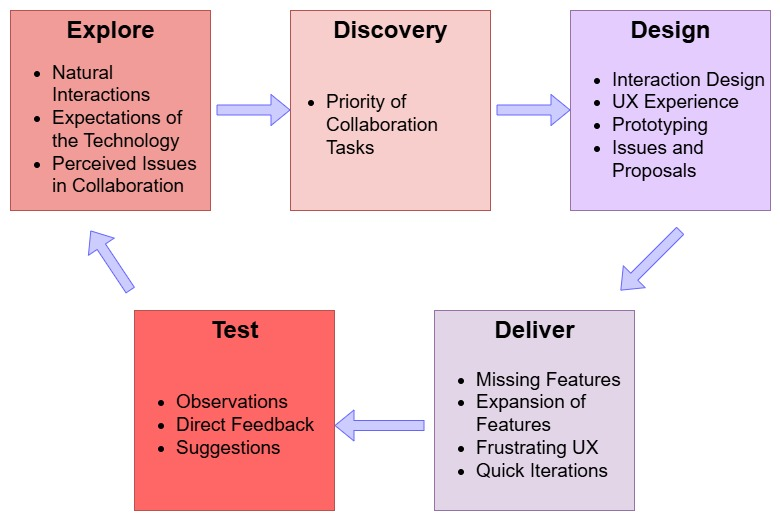
\includegraphics[alt={Figure 3.2},width=0.99\textwidth]{figures/F3-2.jpg}}
    \caption{User Input in the User-Centred Design Process \label{fig:3-2}}
\end{figure}

The biggest risk that needs to be acknowledged when implementing a user-centred design is to mismanage the involvement of the user in the process. As \textcite{wilson_2014}
exemplifies, this situation can take the form of:

\begin{itemize}
    \item A lack of expertise guiding the project, which results in only community-driven ideas than can turn out amateurish in nature or not considering the whole extent
    and context of the project.
    \item A disorganised input that lacks cohesion and a clear goal.
    \item Stumbled progress, usually due to late decision making or relaying on the necessity to please many disjointed voices.
\end{itemize}

The clear goal of creating a shared space for collaborative work and the learning goals for the general software development and the industry project course help in
mitigating these risks. Other guidelines have been established to keep the interaction design focused and to help the analysis and incorporation of feedback in the
different stages of the process:

\begin{itemize}
    \item The development of \emph{WorkshopAR} is mobile-first. Several aspects of multiplatform interactions will be discussed and tested, but the priority in design will be
    given to the technology and input methods found primarily in mobile environments, leveraging the handholds and methods present and expected in the medium.
    \item The main design space will be in 3D interactions and the use of \ac{AR} to solve problems like the selection of objects, positioning and image identification.
    Aesthetical decisions and design are important but not the focus of the research.
    \item \ac{AR} is a new interaction space for many users, but plenty of sources have shown and tested different designs with positive results. The design guidelines for
    \ac{AR} interactions developed by Google DevWorks \parencite{arcore_2025} are a good example of the available solutions in the current market than can be leveraged and
    expanded upon without the necessity of reinventing the wheel.
\end{itemize}

This philosophy behind the user-centred design was also used as part of the iterative process for the software development, especially in support of the analysis and
testing steps, as will be described in the next section.

\subsubsection{Software Engineering Process \label{sec:3-3-2-2}}

The process proposed for this development is based on the stages and activities recommended by \textcite{salo_2007} to conduct and agile development process that is
constantly checking for improvement and for effective use of resources. The research context in which \emph{WorkshopAR} is developed, and the exploratory nature of the objectives
behind the software proposal require for the approach of the development process to be flexible and agile.

The process will be used in the context of a development that tries to deliver functionality fast and in increasing complexity. This behaviour is a response to the
necessity of tentatively explore solutions for the educational and technological challenges of the project, to change course, pivot a proposal and be able to incorporate
the input of the user participation as explored in the previous section.

As \textcite{elbanna_2016} explains, agile developments are useful for getting unrestrictive progress in rapidly changing environments, but they run the risk of aimlessly
keep producing bloated functionalities and lack a clear direction. For the prototyping nature of \emph{WorkshopAR}, this is an acceptable use scenario, and the same guidelines
established to focus the user-centred design process can be used to guide the software development. Additional milestones can also be proposed to evaluate progress and to
set a baseline of what can be considered a finished version of \emph{WorkshopAR} within the context of the project.

\begin{displayquote}
    Milestone 1: A multiuser experience with shared visuals and coordinated interactions.
\end{displayquote}

\begin{displayquote}
    Milestone 2: Visualisation of relevant digital constructs for the learning activities and varied interactions with them in a 3D space.
\end{displayquote}

\begin{displayquote}
    Milestone 3: Tools for communication and team management.
\end{displayquote}

These milestones are general enough that allow movement and flexibility around the objectives to achieve, but they also offer specific criteria to determine if an idea or
proposal is outside the development scope.

Time constrains are also an effective tool to avoid an iterative process to spiral indefinitely \parencite{waldmann_2011,kula_2022}. The nature of the research itself
establishes a hard time constraint for the development that needs to consider access to the case study and the work needed for the research outside the software development.
Figure \ref{fig:3-3} shows the top-level structure of the development process that contemplates the research and evaluation steps done before and after the development, as
well as the need to fit the process with the schedule of the case study.

\begin{figure}[t]
    \centering{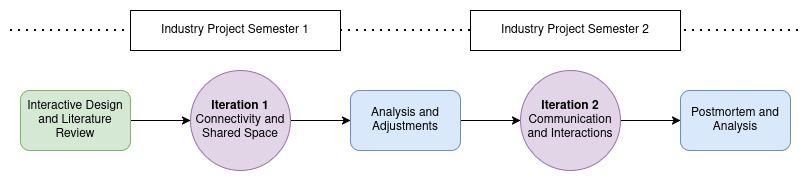
\includegraphics[alt={Figure 3.3},width=0.99\textwidth]{figures/F3-3.jpg}}
    \caption{Top Structure of the Development Process \label{fig:3-3}}
\end{figure}

For the timeframe at hand, it was considered possible to divide the development process into two iterations aimed at two complementary objectives. The first iteration
could build upon the previous literature review and early design stages and increasingly offer different functionalities to the users throughout iteration 2. This model
also takes advantage of the flow of the case study that proposes a similar structure and is also iterative in nature.

Each iteration establishes clear requirements and runs through the process several times, gathering user feedback to determine if it can derive in a meaningful change or
needs to be tackled in the next iteration. Figure \ref{fig:3-4} shows in more detail these dynamics in a single iteration.

\begin{figure}[t]
    \centering{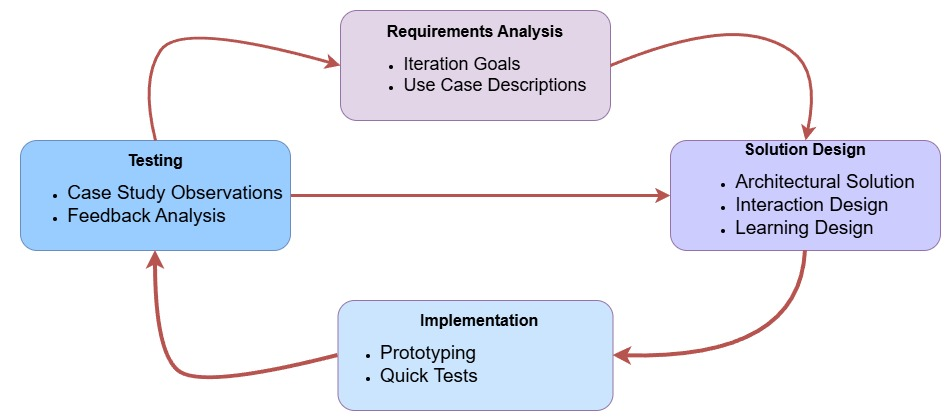
\includegraphics[alt={Figure 3.4},width=0.99\textwidth]{figures/F3-4.jpg}}
    \caption{Activity Flow of an Iteration \label{fig:3-4}}
\end{figure}

\section{Conclusions \label{sec:3-4}}

This chapter has identified and described the major decisions taken for the methodological framework of this research. The strategy proposed is based on a quantitative
approach that focuses on exploring the topic of \ac{CL} using \ac{AR} through two complementary perspectives:

\begin{itemize}
    \item An learning design that establishes clear objectives for the development of the \ac{TEL} intervention. These objectives are meant to develop fundamental skills
    for effective teamwork and communication and are based in strong educational approaches of social constructionism and good teaching practices for adult learners.
    \item An exploratory software development aimed at proposing solutions to challenges of interaction design for shared \ac{AR} experiences. It also needs to propose
    effective mechanisms to properly integrate itself with the learning design of the target course. This software is developed through an iterative approach that is
    centred on user feedback, quick adjustments and fast delivery.
\end{itemize}

The theoretical background explained supports the main objective of this research of integrating a strong learning design in the implementation of a mobile technology
intervention in the classroom.

The next step is to describe the results of applying the experiences and ideas gathered through the literature and in the methodological guidelines, first in the design and
development that supported the technological approach of the intervention, an then in its use during the interaction with the Industry Project course.